\documentclass[t]{beamer}
\usetheme{iclpt}
\nonstopmode

\author{Robert Kruszewski}
\title[Accelerating agent-based Python models]{Accelerating agent-based Python models}

\usepackage[T1]{fontenc}
\usepackage{lmodern}
\usepackage{tabularx, alltt, amsmath, multirow, graphicx, url, graphics, caption, natbib, listings, fancyhdr, lstlinebgrd, etoolbox, todonotes, colortbl}

\lstdefinelanguage[GNU99]{C}[99]{C}
  {morekeywords={asm,__asm__,__extension__,typeof,__typeof__}%
  }%

\lstdefinelanguage[99]{C}%
  {morekeywords={_Bool,_Complex,_Imaginary,auto,break,case,char,%
      const,continue,default,do,double,else,enum,extern,float,for,%
      goto,if,inline,int,long,register,restrict,return,short,signed,%
      sizeof,static,struct,switch,typedef,union,unsigned,void,volatile,%
      while},%
   sensitive,%
   morecomment=[s]{/*}{*/},%
   morecomment=[l]//,%
   morestring=[b]",%
   morestring=[b]',%
   moredelim=*[directive]\#,%
   moredirectives={define,elif,else,endif,error,if,ifdef,ifndef,line,%
      include,pragma,undef,warning}%
  }[keywords,comments,strings,directives]%

\definecolor{lightgray}{rgb}{0.83, 0.83, 0.83}
\definecolor{gray}{rgb}{0.5, 0.5, 0.5}
\definecolor{white}{rgb}{1, 1, 1}
\definecolor{lightcarminepink}{rgb}{0.9, 0.4, 0.38}
\definecolor{babyblue}{rgb}{0.54, 0.81, 0.94}

\definecolor{cython-line-1}{rgb}{1,1,0.28}
\definecolor{cython-line-2}{rgb}{1,1,0.91}
\definecolor{cython-line-3}{rgb}{1,1,0.13}
\definecolor{cython-line-4}{rgb}{1,1,0.59}
\definecolor{cython-line-5}{rgb}{1,1,0.83}

\lstset{
  basicstyle=\ttfamily,                   % Code font, Examples: \footnotesize, \ttfamily
  keywordstyle=\color{lightcarminepink},        % Keywords font ('*' = uppercase)
  commentstyle=\color{gray},              % Comments font
  numbers=left,                           % Line nums position
  numberstyle=\small\color{gray},                      % Line-numbers fonts
  stepnumber=1,                           % Step between two line-numbers
  numbersep=8pt,                          % How far are line-numbers from code
  backgroundcolor=\color{white}, % Choose background color
  frame=l,
  framerule=1.8pt,                             % A frame around the code
  xleftmargin=0em,
  framexleftmargin=1.7em,
  tabsize=4,                              % Default tab size
  captionpos=t,                           % Caption-position = bottom
  breaklines=true,                        % Automatic line breaking?
  breakatwhitespace=false,                % Automatic breaks only at whitespace?
  showspaces=false,                       % Dont make spaces visible
  showtabs=false,                         % Dont make tabls visible
  columns=fullflexible,                       % Column format
}

\begin{document}
\frame{\maketitle}


\begin{frame}
	\frametitle{\huge Marine ecosystem modelling}
		\LARGE
		\begin{itemize}
			\item Metamodel
			\item Model
			\item Environment
		\end{itemize}
\end{frame}


\begin{frame}[c]

\noindent\begin{minipage}{.45\textwidth}

\begin{figure}[H]
  \begin{center}
    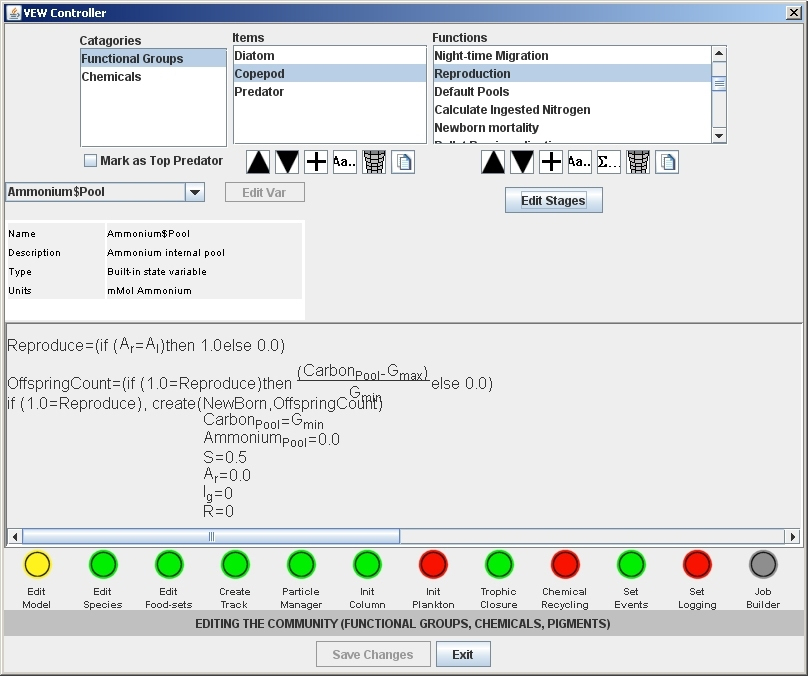
\includegraphics[width=\textwidth,natwidth=808,natheight=676]{images/vew2007-10.jpg}
    \caption{VEW model specification GUI}
  \end{center}
\end{figure}

\end{minipage}\hfill
\begin{minipage}{.45\textwidth}

\begin{figure}[H]
  \begin{center}
    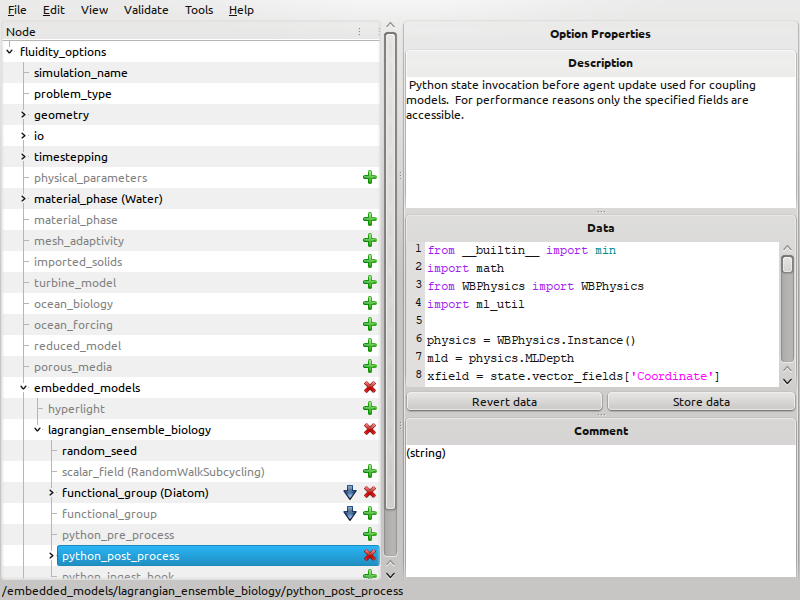
\includegraphics[width=\textwidth,natwidth=800,natheight=600]{images/diamond.png}
    \caption{Fluidity model specification GUI}
  \end{center}
\end{figure}

\end{minipage}
\end{frame}


\begin{frame}[c]

\begin{center}
{\fontsize{48pt}{1em}\selectfont DEMO}
\end{center}

\end{frame}


\begin{frame}
\frametitle{VEW vs Fluidity}
\Large Virtual Ecology Workbench (VEW) \normalsize
\begin{itemize}
	\item One-dimensional physical environment.
	\item Uses Planktonica (DSL) for model specification.
	\item Widely tested and optimised
\end{itemize}
\vspace{12pt}
\Large Fluidity \normalsize
\begin{itemize}
	\item Three-dimensional environment
	\item Uses Python for model specification
	\item Gives VEW complain results, defies optimisation
\end{itemize}
\Large Both use Lagrangian Ensemble (LE) metamodel.
% # Begin with DEMO

% ## THIS HAS TO TAKE 2 MINUTES (RECORD VIDEO OF SIMULATIONS)
% 1. Start a version that takes exactly 2 minutes and start speaking
% 2. Talk about VEW and 1D physics -> why Fluidity is a better solution for the future
% 3. Fluidity is slow - really slow -> Why?
% 4. We have a more sophisticated system but cannot use it in practice
% 5. Can we solve it -> probably, here's a possible solution that works
% 6. It can be done better -> why no one did?
% 7. Launch the same simulation as in point 1. but optimised so they both finish at the same time

% # Describe VEW and Fluidity (2-3 slides tops)
% ## What are the differences

\end{frame}


\begin{frame}[c]

\begin{figure}[H]
  \begin{center}
    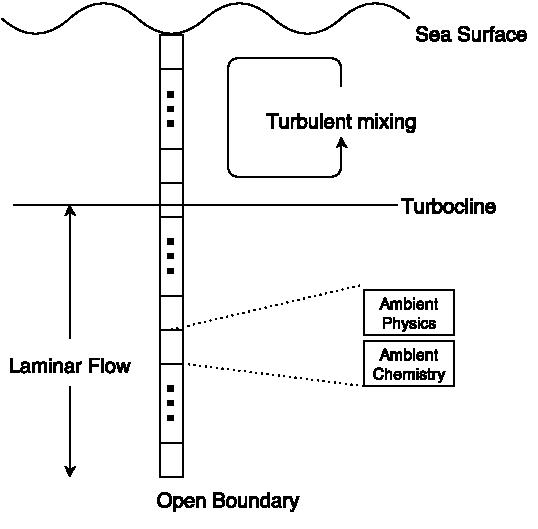
\includegraphics[width=0.6\textwidth,natwidth=473,natheight=466]{images/env-diagram.pdf}
  \end{center}
\end{figure}

\end{frame}


\begin{frame}[c]

\begin{figure}[H]
  \begin{center}
    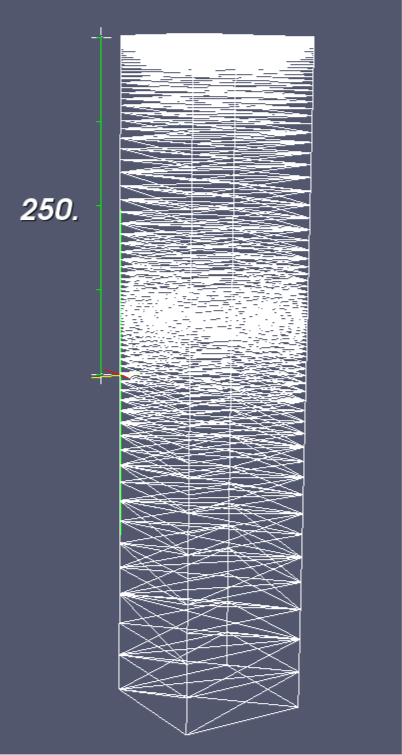
\includegraphics[height=0.9\textheight,natwidth=402,natheight=755]{images/fluidity-mesh.jpg}
  \end{center}
\end{figure}

\end{frame}


\begin{frame}[fragile,t]
\frametitle{\huge Cython}
\noindent\begin{minipage}{.45\textwidth}
\begin{lstlisting}[
  caption=Python code annotated by cython,
  label=list:python-annot,
  language=python,
  linebackgroundcolor={
    \ifnumequal{\value{lstnumber}}{1}{\color{cython-line-1}}{}
    \ifnumequal{\value{lstnumber}}{2}{\color{cython-line-2}}{}
    \ifnumequal{\value{lstnumber}}{3}{\color{cython-line-3}}{}
    \ifnumequal{\value{lstnumber}}{4}{\color{cython-line-4}}{}
    \ifnumequal{\value{lstnumber}}{5}{\color{cython-line-5}}{}
}]
def sumTo(num):
    c = 0
    for i in range(num + 1):
        c = c + i
    return c

\end{lstlisting}
\end{minipage}\hfill
\begin{minipage}{.45\textwidth}
\begin{lstlisting}[
  caption=Sample Cython code,
  label=list:python-cython,
  language=python
]
cpdef int sumTo(int num):
    cdef int c = 0
    cdef int i
    for i in range(num + 1):
        c = c + i
    return c
\end{lstlisting}
\end{minipage}
\end{frame}


\begin{frame}[fragile,c]
\frametitle{\huge Challenge}
\begin{lstlisting}[
	language=python,
	caption=Python version
]
  Q_N = (vars['Ammonium'] + vars['AmmoniumIngested'] + vars['Nitrate'] + vars['NitrateIngested']) / vars['Carbon']
\end{lstlisting}

\begin{lstlisting}[
	language=c,
	caption=C version
]
float Q_N = (vars[AMMONIUM_POOL] + vars[AMMONIUM_ING] + vars[NITRATE_POOL] + vars[NITRATE_ING]) / vars[CARBON_POOL];
\end{lstlisting}

\end{frame}


\begin{frame}[fragile,c]

\frametitle{\huge Python embedding}
\begin{lstlisting}[language=c]
#include <Python.h>
#include "modulename.h"

void cython_call() {
    Py_Initialize();
    initmodulename();
    ... call functions from "modulenam"
    Py_Finalize();
}
\end{lstlisting}

\end{frame}

\begin{frame}[fragile,c]

\frametitle{\huge Array wrappers}
\begin{lstlisting}[language=python]
cdef class AgentWrapper:

    cdef float * array

    def __getitem__(self, key):
        return self.array[agentNames[key]]

    def __setitem__(self, key, value):
        self.array[agentNames[key]] = value
\end{lstlisting}
\end{frame}


\begin{frame}[c]

\begin{figure}[ht!]
  \begin{center}
    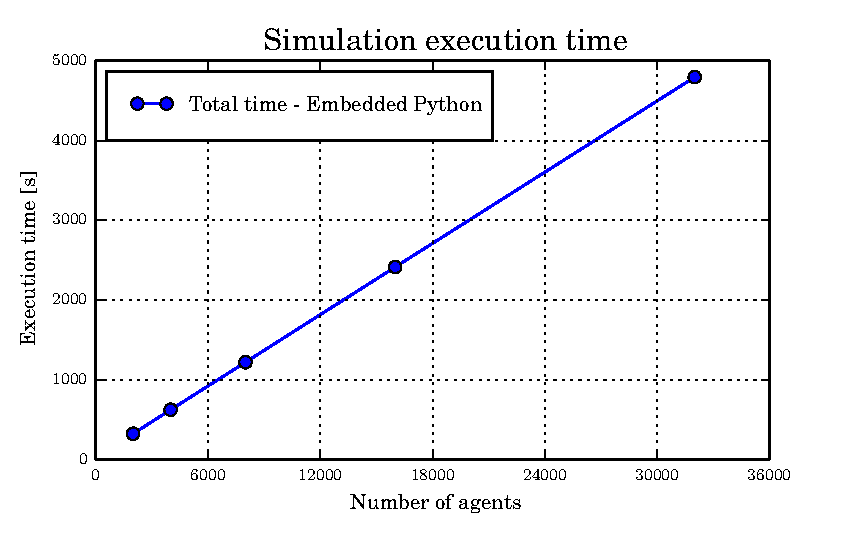
\includegraphics[width=\columnwidth]{graphs/cython-perf.eps}
  \end{center}
\end{figure}

\end{frame}


\begin{frame}[c]

\begin{figure}[ht!]
  \begin{center}
    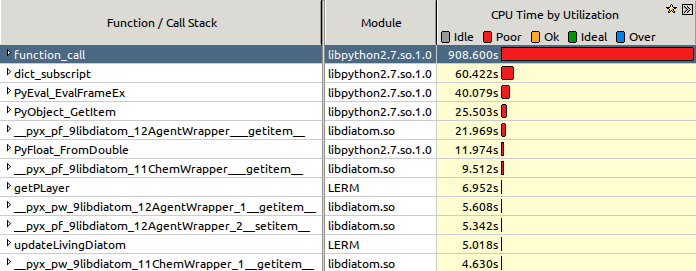
\includegraphics[width=\textwidth,natwidth=696,natheight=271]{images/vtune-cython-pure.png}
  \end{center}
\end{figure}

\end{frame}


\begin{frame}[c]
	\small
	\begin{table}
	    \begin{tabular}{|c|c||c|}
	    \hline
	    Function                      & Module              & CPU Time [s]  \\ \hline
	    \rowcolor{babyblue}
	    dict\_subscript               & libpython2.7.so.1.0 & 59.322        \\
	    \rowcolor{babyblue}
	    PyNumber\_Multiply            & libpython2.7.so.1.0 & 56.8798       \\
	    \rowcolor{babyblue}
	    PyObject\_GetItem             & libpython2.7.so.1.0 & 40.8782       \\
	    \rowcolor{babyblue}
	    PyNumber\_Add                 & libpython2.7.so.1.0 & 39.6466       \\
	    \_update\_Living\_Diatom      & lerm\_diatom.so     & 37.4249       \\
	    \rowcolor{babyblue}
	    PyNumber\_Divide              & libpython2.7.so.1.0 & 28.8877       \\
	    \rowcolor{babyblue}
	    PyObject\_RichCompare         & libpython2.7.so.1.0 & 23.3954       \\
	    \rowcolor{babyblue}
	    PyDict\_GetItem               & libpython2.7.so.1.0 & 20.917        \\
	    \rowcolor{babyblue}
	    float\_dealloc                & libpython2.7.so.1.0 & 16.3916       \\
	    \rowcolor{babyblue}
	    PyFloat\_FromDouble           & libpython2.7.so.1.0 & 15.1369       \\
	    AgentWrapper\_\_\_getitem\_\_ & libdiatom.so        & 11.7308       \\
	    \rowcolor{babyblue}
	    PyNumber\_Subtract            & libpython2.7.so.1.0 & 9.96057       \\
	    math\_pow                     & libpython2.7.so.1.0 & 9.27262       \\
	    math\_1                       & libpython2.7.so.1.0 & 7.66173       \\ \hline
	    \end{tabular}
	    \label{table:vtune-embedded-profile}
	\end{table}
\end{frame}


\begin{frame}[c]
	\begin{figure}[H]
	    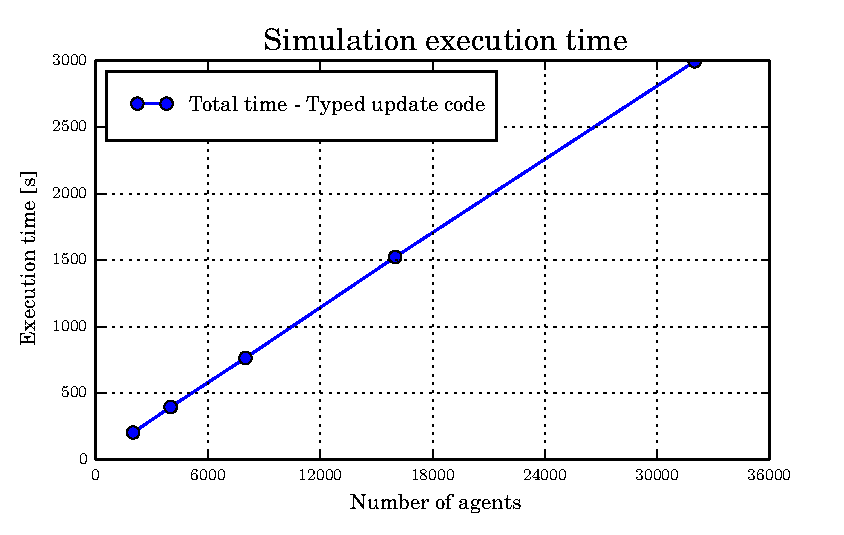
\includegraphics[width=\columnwidth]{graphs/cython-typed-perf.eps}
	\end{figure}
\end{frame}


\begin{frame}
	\frametitle{\huge Threading Python}
	\Large
	\begin{itemize}
		\item Python is truly parallel - all threads are native OS threads.
		\item There should be no limits to parallelising Python code.
		\item Python provide libraries to facilitate thread and process level parallelism.
		\item CPython has Global Interpreter Lock.
	\end{itemize}
\end{frame}


\begin{frame}
	\frametitle{\huge Global Interpreter Lock (GIL)}
	\Large
	\begin{itemize}
		\item You do not talk about the GIL.
		\item You do NOT talk about the GIL.
	\end{itemize}
	\pause
	\begin{itemize}
		\item Used for garbage collection.
		\item Exclusive lock for modifying interpreters state.
		\item Ensures correct reference counts on interpreter objects.
		\item Renders Python effectively single threaded.
	\end{itemize}
\end{frame}


\begin{frame}[fragile,c]
\frametitle{\huge Avoiding GIL}
\begin{lstlisting}[language=c++]
class ArrayMap {
    private V * dataArray;
    private std::unordered_map<K, size_t> dataMap;

    public V& operator[](const K&);
};

V& ArrayMap<K, V>::operator[](const K& key) {
    return this->dataArray[this->dataMap[key]];
};
\end{lstlisting}
\end{frame}


\begin{frame}[c]
	\frametitle{C++ Wrappers}
	\begin{figure}[H]
	  \begin{center}
	    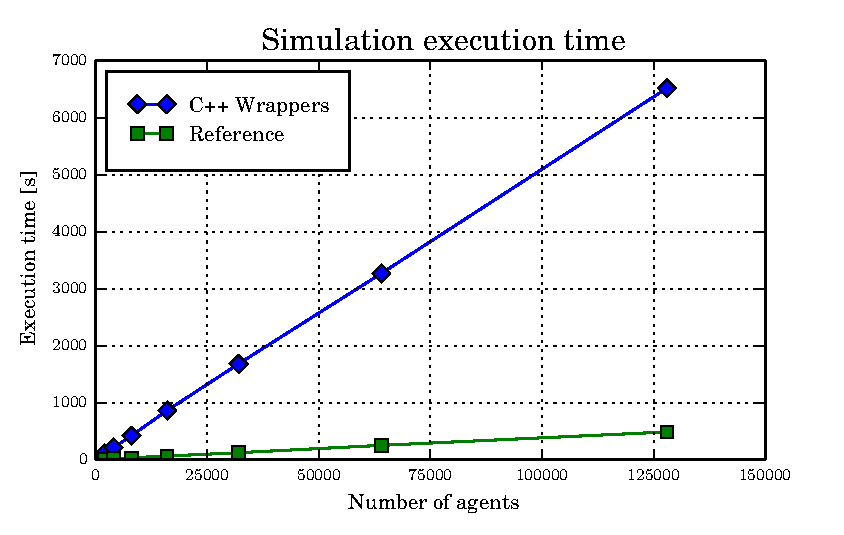
\includegraphics[width=0.9\columnwidth]{graphs/gil-free-perf.eps}
	  \end{center}
	\end{figure}
\end{frame}


\begin{frame}[c]
	\begin{figure}[H]
	  \begin{center}
	    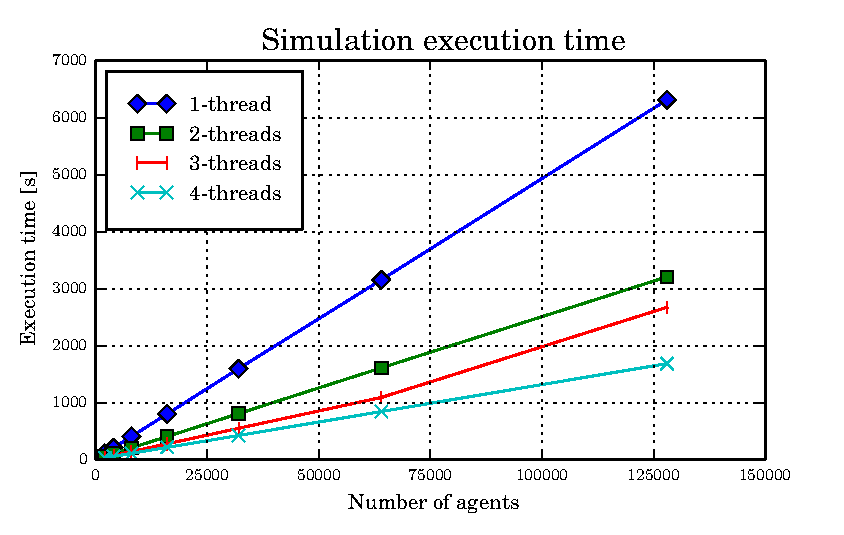
\includegraphics[width=\columnwidth]{graphs/gil-free-multi-4-perf.eps}
	  \end{center}
	\end{figure}
\end{frame}


\begin{frame}[c]
	\small
	\begin{table}
	    \begin{tabular}{|c|c||c|}
	    \hline
	    Function                                 & Module              & CPU Time               \\ \hline
	    \rowcolor{babyblue}
	    \_M\_find\_before\_node                  & lerm\_diatom.so     & 58.9617 \\
	    \rowcolor{babyblue}
	    std::\_Hash\_bytes                       & libstdc++.so.6.0.20 & 42.4008  \\
	    \rowcolor{babyblue}
	    \_M\_find\_before\_node                  & lerm\_diatom.so     & 35.9007 \\
	    \rowcolor{babyblue}
	    operator==\textless char\textgreater     & lerm\_diatom.so     & 15.5598 \\
	    \rowcolor{babyblue}
	    \_\_memcmp\_sse4\_1                      & libc-2.19.so        & 14.8557         \\
	    \rowcolor{babyblue}
	    \_S\_equals                              & lerm\_diatom.so     & 9.29432 \\
	    \rowcolor{babyblue}
	    std::\_\_detail::\_Map\_base::operator[] & lerm\_diatom.so     & 9.15494 \\
	    \rowcolor{babyblue}
	    operator()                               & lerm\_diatom.so     & 8.44585 \\
	    lerm\_diatom\_update\_Living\_Diatom     & lerm\_diatom.so     & 8.33352 \\
	    \_\_pow                                  & libm-2.19.so        & 5.9977          \\
	    \rowcolor{babyblue}
	    operator==\textless char\textgreater     & lerm\_diatom.so     & 5.47811 \\
	    \rowcolor{babyblue}
	    \_S\_equals                              & lerm\_diatom.so     & 4.67876 \\
	    \_\_exp                                  & libm-2.19.so        & 4.06897       \\ \hline
	    \end{tabular}
	\end{table}
\end{frame}


\begin{frame}[fragile,c]
\frametitle{\huge Use arrays}
\begin{lstlisting}[
	language=python,
	caption=Cython with C arrays
]
cdef float Q_N = (vars[1] + vars[0] + vars[7] + vars[6]) / vars[4]
\end{lstlisting}

\begin{lstlisting}[
	language=c,
	caption=Reference C version
]
float Q_N = (vars[AMMONIUM_POOL] + vars[AMMONIUM_ING] + vars[NITRATE_POOL] + vars[NITRATE_ING]) / vars[CARBON_POOL];
\end{lstlisting}
\end{frame}


\begin{frame}[c]
	\begin{figure}[H]
	  \begin{center}
	    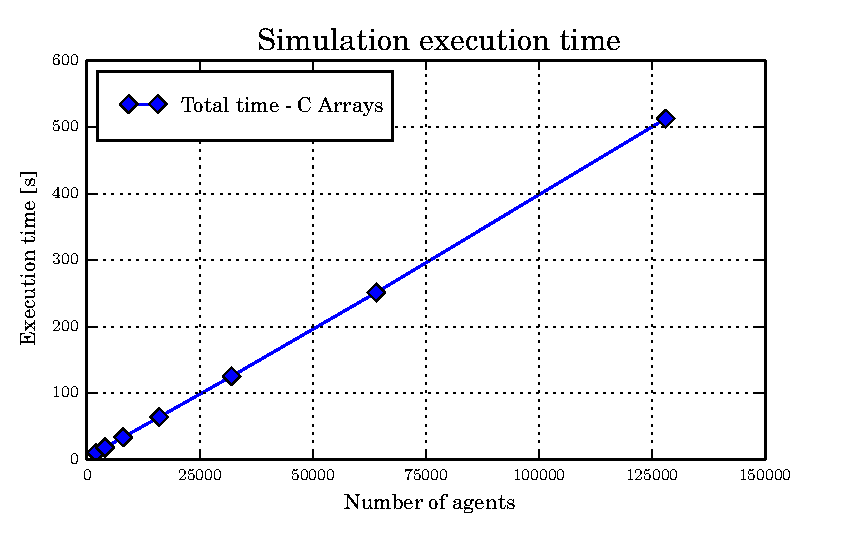
\includegraphics[width=\columnwidth]{graphs/dict-array-perf.eps}
	  \end{center}
	\end{figure}
\end{frame}


\begin{frame}[c]
	\begin{figure}[H]
	  \begin{center}
	    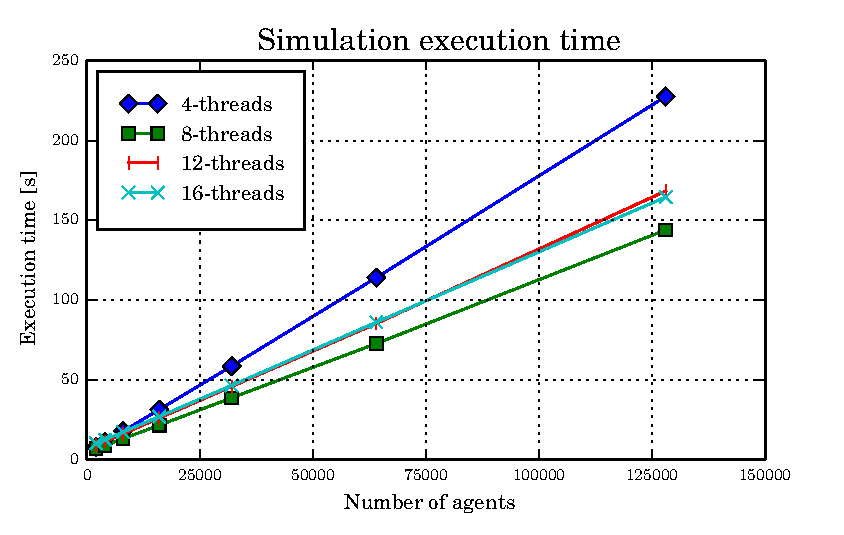
\includegraphics[width=\columnwidth]{graphs/dict-array-multi-16-perf.eps}
	  \end{center}
	\end{figure}
\end{frame}


\begin{frame}[c]
	\frametitle{Correctness}
	\begin{figure}[H]
	  \begin{center}
	    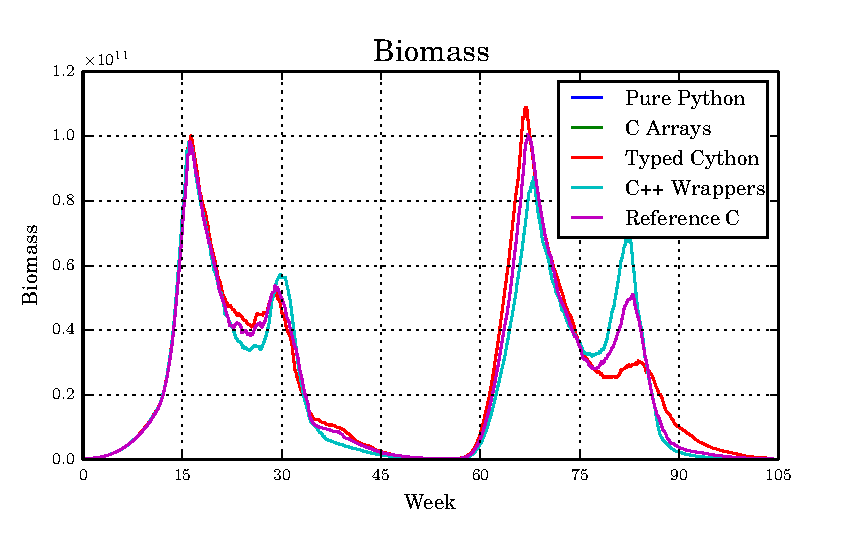
\includegraphics[width=0.9\columnwidth]{graphs/bio-fixed-single-float-comp.eps}
	  \end{center}
	\end{figure}
\end{frame}


\begin{frame}[c]
	\begin{figure}[H]
	  \begin{center}
	    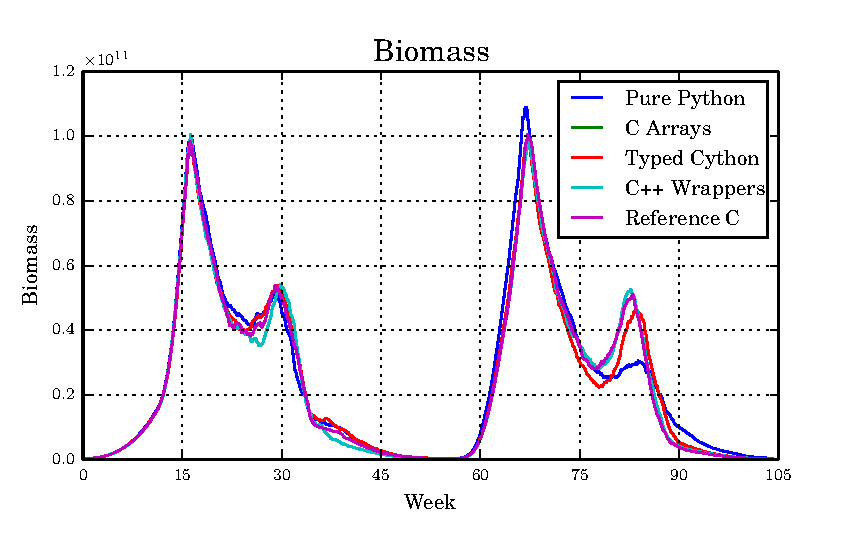
\includegraphics[width=\columnwidth]{graphs/bio-fixed-single-double-comp.eps}
	  \end{center}
	\end{figure}
\end{frame}


\begin{frame}[c]
	\frametitle{Summary}
	\begin{figure}[H]
	  \begin{center}
	    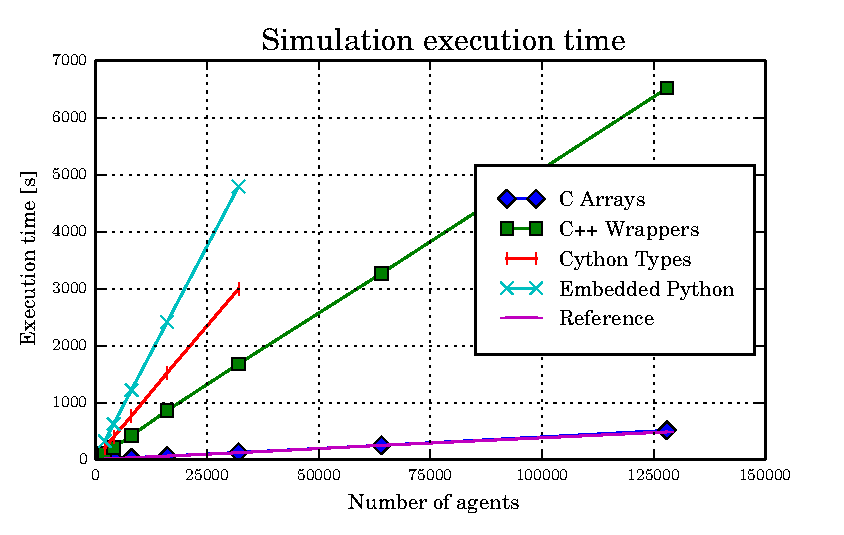
\includegraphics[width=0.9\columnwidth]{graphs/compared-single-perf.eps}
	  \end{center}
	\end{figure}
\end{frame}


\begin{frame}[c]
	\begin{figure}[H]
	  \begin{center}
	    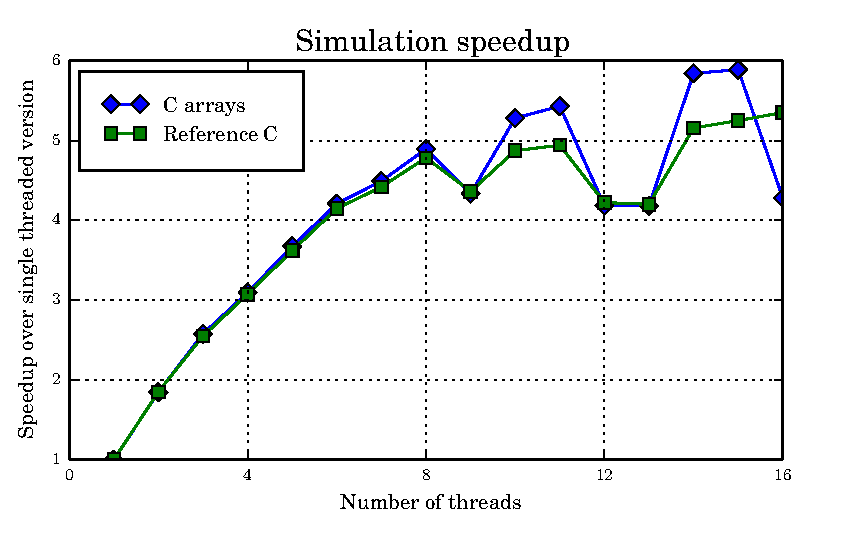
\includegraphics[width=\columnwidth]{graphs/speedup.eps}
	  \end{center}
	\end{figure}
\end{frame}


\begin{frame}[c]

\begin{center}
{\fontsize{60pt}{1em}\selectfont Thank you}
\end{center}

\end{frame}


\begin{frame}[c]

\begin{center}
{\fontsize{48pt}{1em}\selectfont Questions?}
\end{center}

\end{frame}

\end{document}
